%manuel 6e, chapitre G3
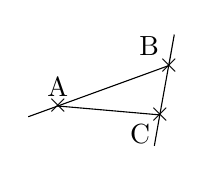
\begin{tikzpicture}[scale=1,every node/.style={scale=1}]

\draw (0,0) node [above]{A};
\draw (0,0) node {$\times$};
\draw (20:1.5) node [above left]{B};
\draw (20:1.5) node {$\times$};
\draw (-5:1.3) node [below left]{C};
\draw (-5:1.3) node {$\times$};

\draw (20:1.5)--+(80:0.4)--(-5:1.3)--+(-100:0.4);
\draw (0,0)--(-5:1.3);
\draw (0,0)--+(200:0.4)--(20:1.5);

\draw (0,0.7); %pour donner un peu plus de hauteur à l'image
\end{tikzpicture} 
